
\newpage
\section{Data Link Layer (Sicherungsschicht)}

\subsection{Layer 2 Aufgaben:}{
    \begin{itemize}[noitemsep]
        \item  Frame Delineation → Präambel und SFD
        \item Fehlererkennung → CRC
        \item  Fehlerkorrektur → bei Ethernet keine auf dem MAC Layer
        \item  Adressierung → global gültige MAC-Adressen
        \item  Media Access Control → CSMA/CD
        \item Master/Slave: Master fragt Slaves ab (Master ist Single Point of Failure)
        \item  Token Passing: Berechtigung wird weitergereicht (Token Management ist aufwendig)
        \item  Zeitgesteuerte Zuteilung des Mediums (aufwendige Planung nötig)
    \end{itemize}
}




\subsection{Framing (Asynchron)}{
\begin{itemize}[noitemsep]
    \item Keine Daten → Nichts wird gesendet
    \item Zu Beginn eines Frames wird ein Start-Bit gesendet
\end{itemize}

{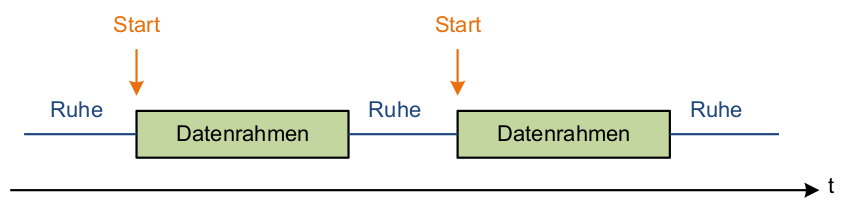
\includegraphics[scale=.3]{img/framing_async.png}}
}

\subsection{Framing (Synchron)}{

    \begin{itemize}[noitemsep]
        \item Frames werden ohne Unterbruch gesendet
        \item Stehen keine Daten an, werden Flags gesendet
        \item Frames werden durch ein Start- und ein End-Flag begrenzt
                  {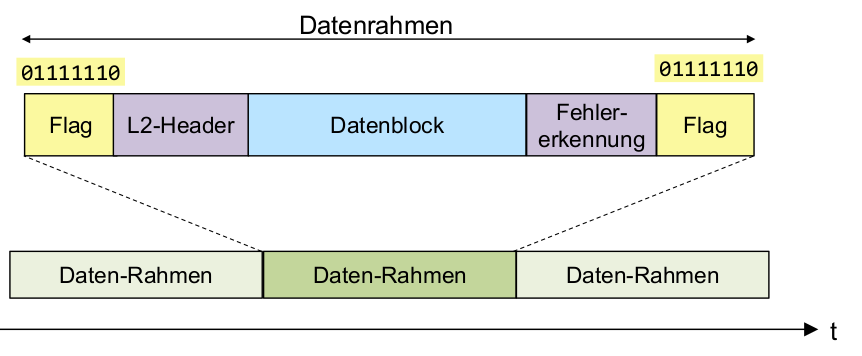
\includegraphics[scale=.275]{img/framing_sync.png}}
    \end{itemize}
}

\subsection{Bitstopfen}{
    Wird verwendet, um ein Bitmuster zu garantieren.

    \begin{itemize}[noitemsep]
        \item Sender fügt im Datenstrom nach 5 Einsen immer eine 0 ein.
        \item Empfänger wirft nach 5 Einsen immer ein Bit weg.
    \end{itemize}
}


\subsection{Fehlererkennung / Fehlerkorrektur}{
    \begin{itemize}[noitemsep]
        \item FER (Frame Error Ratio)
        \item RER (Residual Error Ratio)
        \item BER (Bit Error Ratio) Anzahl fehlerhafte Bits im Verhältnis zu Gesamtzahl der Bits
    \end{itemize}
}



\subsection{Wahl der Framelänge}{
    \begin{itemize}[noitemsep]
        \item Lange Frames $\to$ Höhere Nutzdatenrate, Fehleranfällig
        \item Kurze Frames $\to$ Tiefere Nutzdatenrate, Zuverlässig
    \end{itemize}
}
\subsection{Datenraten}{
    $F_R = FrameRate$,$B=BitRate$,$F_L = FrameLength$ \\
    $ N = NutzBits $,$P = Payload$

    $$ F_R = \frac{B}{8 \cdot (F_L + IFG)} $$
    $$ N = F_R \cdot P \cdot 8 $$
   
}


